% BLM の資産の推移（事前登録の追記 1。検定はせず報告だけ）
\chapter{BLM の資産の推移}\label{ch:blm}

事前登録の追記 1（どの株価の反応も計算する前に追加）：四半期（3・6・9・12 月）・半年（6・12 月）・1 年（12 月）ごとにリバランスする BLM の比率で、2015 年 12 月末と 2023 年 12 月末をそれぞれ 1 とした資産の推移を作った（\code{blm\_paths.py}）。

\begin{itemize}
\item 範囲：各リバランスの日に小型株の範囲にいて、直近 252 日のうち 126 日以上の株価がある会社。
\item 見通し：その日以前に反応日がある、直近 92 日以内の最新の発表の点数を正規スコアにした。BLM は実験 7・9 と同じ形（$\delta = 2.5$、$\tau = 0.025$、He--Litterman の $\Omega$、IC $= 0.05$）で、見通しの大きさは保有期間に合わせた（日次で IC × $\sigma_{\text{日}}$ × $z / \sqrt{h}$）。共分散は直近 252 日の Ledoit--Wolf。事前の TE の上限は年 3\%（校正しない）。
\item 比べる相手：同じ範囲を浮動株時価総額で加重したもの。両方から、売買した額の片道 0.3\% を引いた。
\item \textbf{検定はしない}（事前登録の通り、報告だけ）。
\end{itemize}

\section{2015 年末から}

\begin{table}[H]
\centering\small
\caption{2015 年 12 月末を 1 とした資産の推移（2026 年 9 月末まで）。年率と相手との差は年率、実現の TE は年率、回転率はリバランス 1 回あたり}
\label{tab:blm2015}
\tabin{blm_2015}
\end{table}

\begin{figure}[H]
\centering
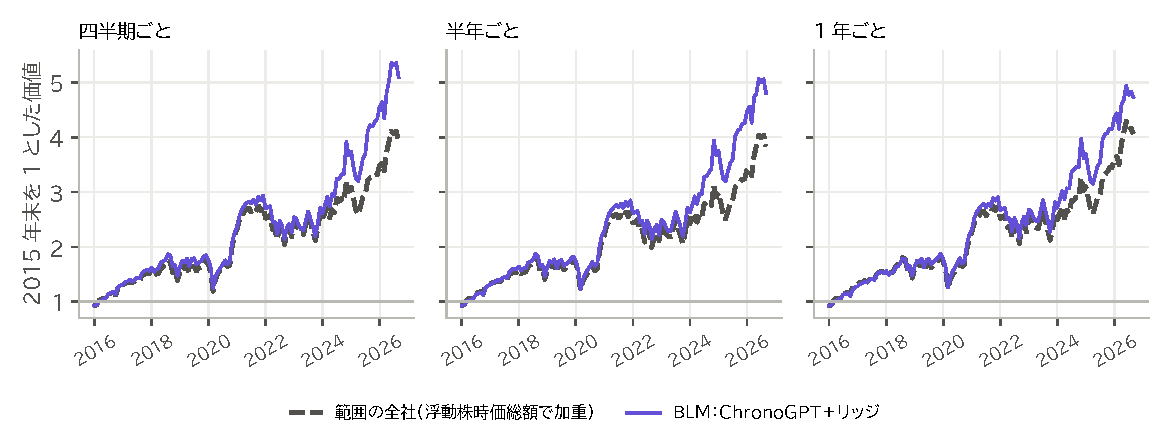
\includegraphics[width=\linewidth]{blm_2015.pdf}
\caption{2015 年末を 1 とした推移。BLM は ChronoGPT＋リッジの見通し。}
\label{fig:blm2015}
\end{figure}

\section{2023 年末から}

\begin{table}[H]
\centering\small
\caption{2023 年 12 月末を 1 とした資産の推移（2026 年 9 月末まで、約 2 年 9 か月）}
\label{tab:blm2023}
\tabin{blm_2023}
\end{table}

\begin{figure}[H]
\centering
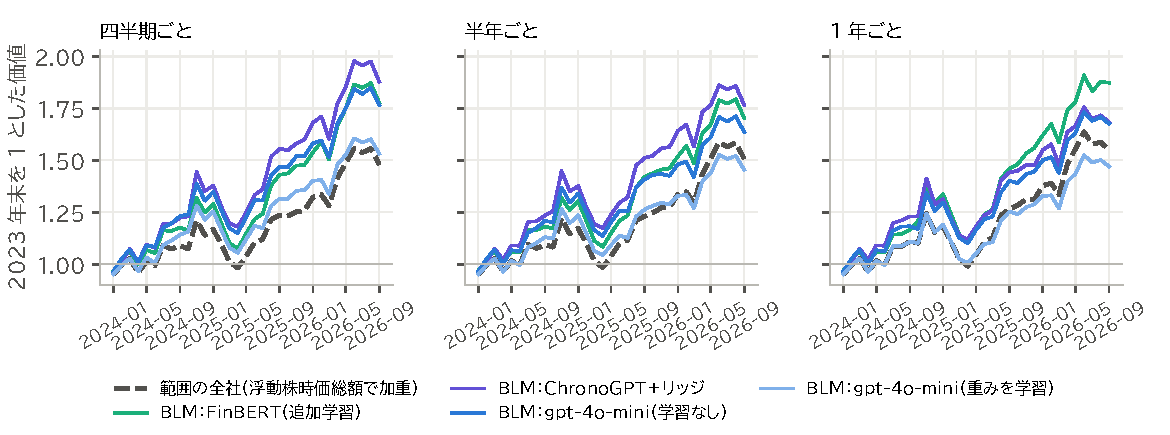
\includegraphics[width=\linewidth]{blm_2023.pdf}
\caption{2023 年末を 1 とした推移。gpt-4o-mini（重みを学習）は 2024 年の第 1 四半期から点数があり、それ以前の日は見通しなし（範囲の比率）。}
\label{fig:blm2023}
\end{figure}

\section{読み方}

\begin{itemize}
\item \textbf{2015 年末から}：ChronoGPT＋リッジの BLM は、3 つのリバランスの頻度のどれでも、比べる相手を年率で上回った（四半期 \V{B2015quarterchronoridgeex}、半年 \V{B2015halfchronoridgeex}、1 年 \V{B2015yearchronoridgeex}）。最終の値は、四半期で \V{B2015quarterchronoridge}、比べる相手は \V{B2015quarterband}。ただし、\figref{fig:blm2015} のとおり、差の多くは 2023 年以降に開いた。2016〜2022 年は、ほぼ同じ動きだった。
\item \textbf{2023 年末から}：ChronoGPT＋リッジ、FinBERT（追加学習）、gpt-4o-mini（学習なし）の BLM は、どの頻度でも比べる相手を上回った。gpt-4o-mini（重みを学習）は、四半期ではわずかに上回り、半年・1 年では下回った。期間が約 2 年 9 か月と短く、1 年ごとのリバランスは 3 回しかない。
\item \textbf{資産の水準}は、2 本とも生存者バイアスで高く出ている（比べる相手の年率が 13〜17\%）。特に 2015 年からの推移は、範囲の会社の約半分が欠ける時期を含む。意味があるのは、同じ会社の範囲での 2 本の差である。
\item \textbf{実現の TE} は年 3〜7\% 程度で、多くは事前の上限（3\%）を超えた。事前の TE を校正しなかったこと（事前登録で決めた）と、最適化の多くの回で解の精度が「不正確」（\code{optimal\_inaccurate}）と報告されたことによる。不正確と報告された解も、そのまま使った（\code{results/blm\_paths.json} の \code{status}）。
\item \textbf{回帰との関係}：主な検定の予測の力（\chapref{ch:primary}）は、BLM の小さな傾き（TE 数\%）の中で、比べる相手との差として現れた。一方、規模で加重した上位 20\% の月次のポートフォリオ（\chapref{ch:portfolio}）では、有意な差にならなかった。どちらも 1 回の実行の結果であり、BLM の差は検定していない。
\end{itemize}
